\chapter{Introduction}

The code for the whole Project can be found on GitHub via this Link \url{https://github.com/SchoAr/RFM12_Linux}

\section{RFM12}
The RFM12 is a small Radio-Transceiver. The used version is sending and receiving with 433Mhz. The problem with this RF-Module is that it is hardly available any more.\newline
The Data-sheet of the RFM12 can be accessed from here : \url{http://www.hoperf.com/upload/rf/RFM12.pdf}\newline
The Chip uses a frequency shift keying method for sending and receiving. Only a half-duplex communication can be acquired. The whole specification of the chip can be found in the Data sheet and are not discussed in detail.

\begin{figure}[H]
	\centering
		\includegraphics[width=1.00\textwidth]{picture/rfm12.png}
	\caption{RFM12 Chip Pinout}
	\label{fig:rfm12}
\end{figure}

The chip is used with an SPI interface for communication. With an interrupt the Chip indicates if the FIFO is empty in sending mode, or the FIFO received a Byte. Therefore the main program can sleep in receiving mode, until the Interrupt arrives. Also a Byte can be send and the program can do other stuff, until the FIFO is empty and an interrupt occurs.\newline

The Antenna of the Chip has to be designed by one own. The Chip gives a Antenna-pin and a proper Antenna has to be attached on this pin. Therefore the length of the Antenna has to be calculated with the following Formula.

\begin{equation}
	\lambda = \frac{c}{f} = \frac{3\cdot 10^{8}}{433 \cdot 10^{6}} =  692.7mm
\end{equation}

This is the length of a whole wave with the Frequency of 433MHz. Because the whole length is not necessary a $\frac{\lambda}{4}$ Antenna is used.
This is a length of 17,3cm. As a Antenna material a wire, standing up in the air, is used.

\section{Test System}

For a proper test System a receiver had to be chosen. This Board will receive the Messages from the MicroZed Board. I have choose the mbed from \url{mbed.org}. This Board allows a rapid prototyping and users can create specific Library for hardware. The used library for the RFM12 can be found with this link \url{http://developer.mbed.org/users/hajesusrodrigues/code/RFM12B/}\newline

This Library provides basic functions for sending and receiving. It also provides a function for encryption. This is very helpful for sending important data via the ISM Band. But there is a problem with the Library, it is designed for the RFM12B. There are only a few differences but they are important. \newline

\textbf{The First difference is that the RFm12B needs a pull-up Resistor on the PIN FSK/DATA/nFFS. Secondly a special sync byte is needed. This Byte is: 0xD4.}\newline 

Not every Pin of the RFM12 is used. The Used Pins are shown in the following schematic, also visible is the $10k\Omega$ pull-up Resistor.
\begin{figure}[H]
	\centering
		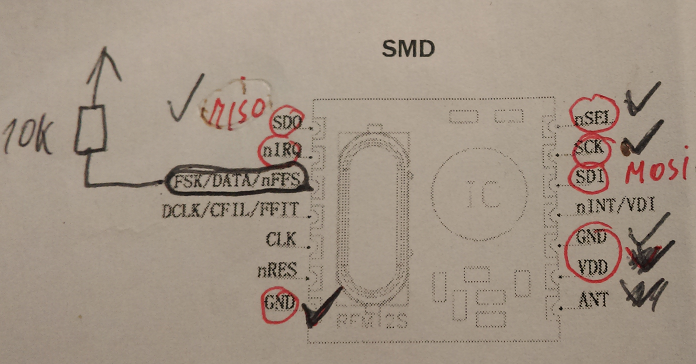
\includegraphics[width=1.00\textwidth]{picture/rfm12_connection.png}
	\caption{Pin out of the RFm12}
	\label{fig:rfm12_pinout}
\end{figure}

Not the real hardware with the Connections is shown in the following picture. One Connection is used as the required Pull up Resistor. The Antenna is not fully visible but standing up in the air.

\begin{figure}[H]
	\centering
		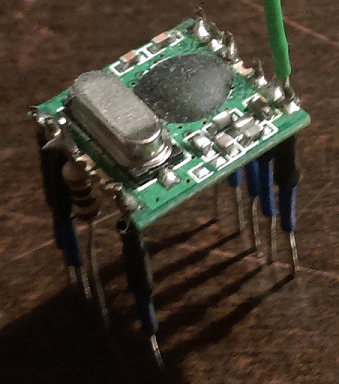
\includegraphics[width=1.00\textwidth]{picture/rfm12_connected.png}
	\caption{RFM12 Chip Connection Wired}
	\label{fig:rfm12_coonnection}
\end{figure}

The mbed test system is build-up on a bread board. The Following picture shows the Board: 

\begin{figure}[H]
	\centering
		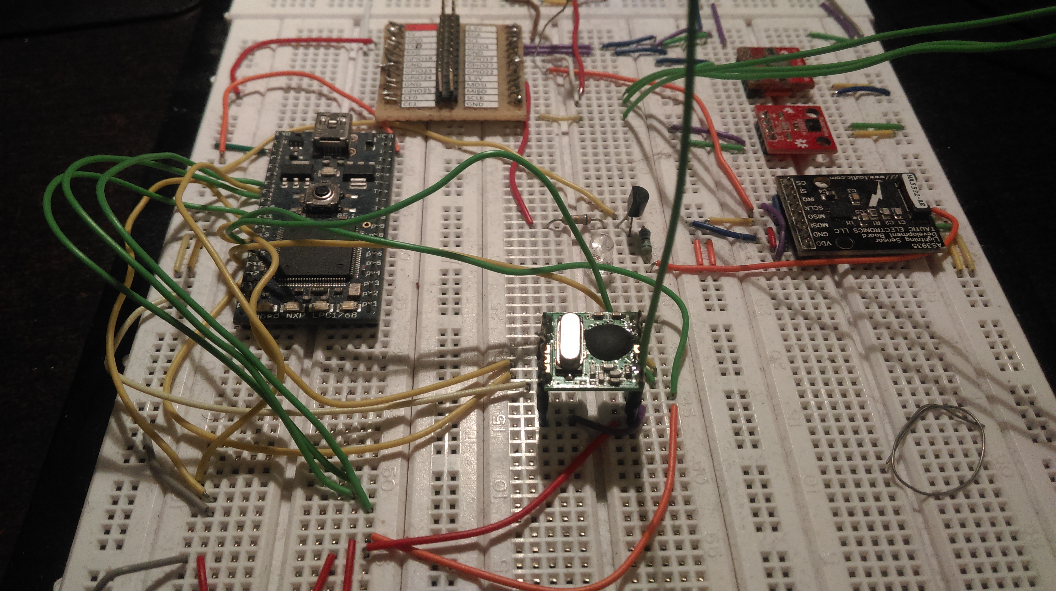
\includegraphics[width=1.00\textwidth]{picture/mbed_build.png}
	\caption{mbed test System}
	\label{fig:rfm12}
\end{figure}

For the connection with the MicroZed Board a special connection Board was Designed. It is a small Board providing the Connection with the RFM12 and 3 LEDs. The blue LED is designed for indicating that the Module is online, and the two green LEDs indicates receiving and transmitting. For Debugging a GND connection is available.

\begin{figure}[H]
	\centering
		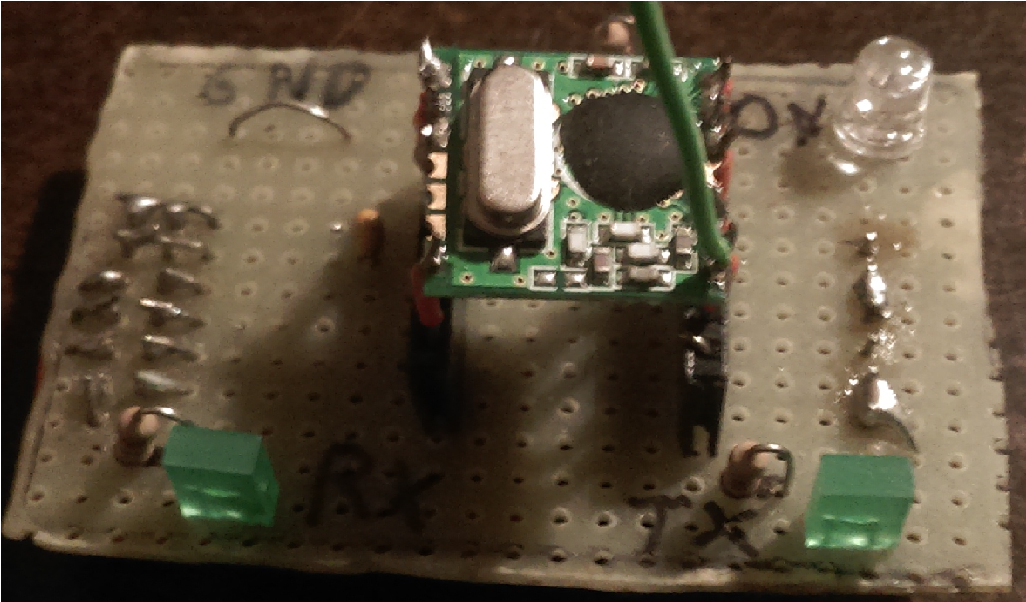
\includegraphics[width=1.00\textwidth]{picture/rfm12_carier.png}
	\caption{Carrier Board}
	\label{fig:rfm12}
\end{figure}

The Connection with the MicroZed Board is designed for the on-board connector. Because then no external Power supply is not required.

\begin{figure}[H]
	\centering
		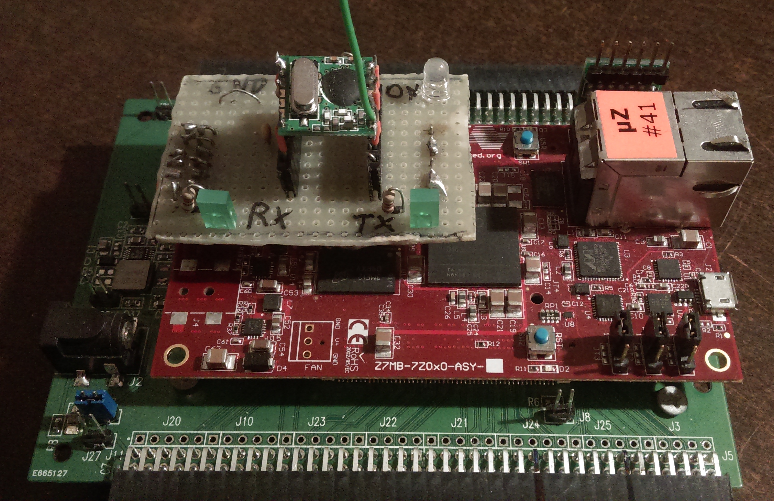
\includegraphics[width=1.00\textwidth]{picture/rfm12_carier_zynq.png}
	\caption{RFM12 connected to the MicroZed Board}
	\label{fig:rfm12}
\end{figure}

The Following table describes the Connection of the RFM12 Carrier board with the MicroZed Board.

\begin{table}[H]
    \centering
    \begin{tabular}{ c | c | c |c}\hline                      
        Connection Name & MIO Pin & Zynq Pin & Connection Type  \\ \hline\hline
        PMOD\_D0 & MIO 13 & E8  & CS \\ \hline
        PMOD\_D1 & MIO 10 & E9  & MOSI \\ \hline
				PMOD\_D2 & MIO 11 & C6  & MISO \\ \hline
				PMOD\_D3 & MIO 12 & D9  & SCLK \\ \hline
				PMOD\_D4 & MIO 0  & E6  & Interrupt \\ \hline
				PMOD\_D5 & MIO 9  & B5  & RX LED \\ \hline
				PMOD\_D6 & MIO 14 & C5  & TX LED \\ \hline
				PMOD\_D7 & MIO 15 & C8  & ON LED \\ \hline
				\hline 
        \end{tabular}
    \caption{Connection Table for Carrier Board}
    \label{tab:Connections}
\end{table}


\section{bare-metal Program for the MicroZed Board}
To test the function of the RFM12 a Bare-metal program was designed. This allows a evaluation of the function. Out of this program the final module was created. Because the mbed was used as counter part for the communication, the Library which is used there was used for creating the MicroZed program. The upper Layer of the communication remains, only the SPI and GPIO layer had to be created new.\newline

\subsection{SPI Bare-metal}
The implementation of the functions on the MicroZed Board are not important,for the module, but it gives an Overview of what the functions should do. The Hole implementation of the bare-metal program can be found on the GitHub Repository: \url{https://github.com/SchoAr/RFM12_Linux/tree/master/BareMetal/src}

\begin{lstlisting}
u16 xfer(u16 cmd) {

	u16 ret;
	u8 TempBufferSend[2];
	u8 TempBufferReceiv[2];
	TempBufferSend[0] = cmd >> 8;
	TempBufferSend[1] = cmd & 0xFF;

	ret = XSpiPs_PolledTransfer(&SpiInstance, TempBufferSend, TempBufferReceiv,
			2);
	if (ret != XST_SUCCESS) {
		printf("[SPI] Error in xfer_16\n");
	}

	ret =  (TempBufferReceiv[0]<<8) | TempBufferReceiv[1];
	return ret;
}
\end{lstlisting}

This function is the most important for the SPI Communication. It is used for writing a 16 bit value to the RFM12 and also receives a 16 bit value.The problem with this function is that the return value is not secured. If the Sending goes wrong only a debug print is given. But this is not very important cause with SPI no acknowledgement System is included like with I²C. In I²C it is possible to check if the counter part is available cause it gives an acknowledgement. For the Initialisation communication a nearly similar function is used, the difference is that the function for the Initialisation doesn't receive any data. \newline

\subsection{GPIO Bare-metal}

After starting a send command the Interrupt Routine controls the States of the RFM12.
\textbf{Very important is that the Interrupt should be triggered with a falling edge.} \newline

The implementation of the Bare-metal program is very simple. With a Initialisation function the GPIO\_Interrupt knows every important parameter. The Initialisation of the GPIO also gets a callback pointer. This function is called if a Interrupt is triggered. In our case this is the Interrupt handler for the RFM12. 
The function call of the initialisation is shown here : \verb|	init_GPIOInterrupt(0, &InterruptHandler, FALLING_EDGE, &gpio, ConfigPtr,&GicInstance);|

The ConfigPtr, gpio and GicInstance are needed for the Xilinx Library, they are only structs for the GPIO and the Global Interrupt Controller. 

\subsection{main fucntion}

In the main Function the RFM12 is initialized, and then in an infinite loop it sends one after another Characters to the mbed. The implementation code is the following: 

\begin{lstlisting}
	while (1) {

		SendStart(SERVER_MBED_NODE, send_message, i, 0,0);
	    (i >= 60) ? i = 0 : i++;
	    delay_s(5);
	}
\end{lstlisting}

The important part here is that the Function SendStart is used to send Data. The Name of the function already Indicates that the sending is not finished when this function returns. The Data is only copied to an internal Buffer and there it is send via the Interrupt. 
